\documentclass[12pt, a4paper]{article}
\usepackage{amsmath}
\usepackage{amsfonts}
\usepackage{amsthm}
\usepackage{mathtools}
\newtheorem{theorem}{Theorem}[section]
\newtheorem{definition}{Definition}[section]
\numberwithin{equation}{section}
\usepackage{pgfplots}
\pgfplotsset{width=10cm,compat=1.9}
\graphicspath{ {img/} }
\DeclareGraphicsExtensions{.png, .jpg}

\title{Singular value decomposition, pseudo-inverses, and principal component analysis}
\author{Kristian Wichmann}

\begin{document}
\maketitle

\section{Gramian matrices}
Given a set of vectors $a_1, a_2,\ldots, a_n\in\mathbb{R}^m$, the Gramian matrix is the traditionally matrix of inner products $\langle a_i,a_j\rangle$. If these vectors are collected into a $m\times  n$ matrix $A$, this matrix can be expressed as $A^t A$. Here, we will use the term for any matrix in this form. By starting out with the transpose instead, this means that $AA^t$ is also a Gramian, with dual results.

\begin{theorem}
\label{gramian_basic}
If $A\in\mathbb{R}^{m\times n}$, then $A^t A$ is symmetric and positive semi-definite. Iff $A$ has rank $m$, $A^t A$ is positive definite.
\end{theorem}
\begin{proof}
$(A^t A)^t=A^t(A^t)^t=A^t A$ shows symmetry. positive semi-definiteness, let $x\in\mathbb{R}^n$. Then:
\begin{equation}
x^t A^t Ax=\langle Ax,Ax\rangle=||Ax||^2
\end{equation}
As a norm, this is greater than or equal to zero. Hence $A^t A$ is positive semi-definite. If $A$ has rank $m$ the map $x\mapsto Ax$ has a trivial kernel by the rank-kernel theorem. Which means only the zero vector is mapped to zero, and hence $A^t A$ is positive definite. If the rank is less than $m$, the kernel is non-trivial and positive definiteness cannot be true.
\end{proof}

\section{The rank-nullity theorem}

\subsection{For $A$ and $A^t$}
According to the rank-nullity theorem, for a matrix $A\in\mathbb{R}^{m\times n}$, the sum of the rank and nullity is $n$. So, if the rank of $A$ is $r$, then $\textrm{null}A=n-r$. Applying the theorem to $A^t$, which also has rank $r$, we get $\textrm{null}A=m-r$.

The image of $A$ is also called the \textit{column space} of $A$, denoted $C(A)$. The image of $A^t$ is also called the \textit{row space} of $A$, $C(A^t)$. The null space of $A^t$ is often called the \textit{left null space}.

\begin{figure}
\centering
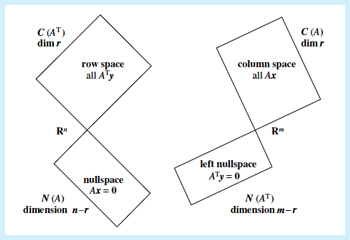
\includegraphics[width=\textwidth]{row_column_null}
\caption{Visualization of dimensionality for the rank-nullity theorem}
\label{fig:rank-nullity}
\end{figure}

These relationships are visualized in figure \ref{fig:rank-nullity}.

\section{Singular value decomposition}

\subsection{Construction and intuition}
We know that the dimensions of the row and column spaces of a matrix $A\in\mathbb{R}^{m\times n}$ are the same, $r$. We now seek out orthonormal bases of each of these spaces - $u_1,u_2,\ldots,u_r$ for column space and $v_1,v_2,\ldots,v_r$ for row space, such that
\begin{equation}
Av_i=\sigma_i u_i
\end{equation}
The sigmas are known as \textit{singular values} for $A$. Now, expand the orthonormal bases to include the null spaces. This means that $Av_i=0$ for $r<i\le n$. In matrix form this means:
\begin{equation}
AV=U\Sigma
\end{equation}
Here, the columns of $U$ and $V$ are made from the respective bases, so $U\in\mathbb{R}^{m\times m}, V\in\mathbb{R}^{n\times n}$, and $\Sigma\in\mathbb{R}^{m\times n}$ is a diagonal $n\times n$ matrix with the $\sigma_i$'s in the first $r$ places of the diagonal and zeroes in the rest. Solving for $A$ we get:
\begin{equation}
A=U\Sigma V^t
\end{equation}
Here we have used that orthogonal matrices are invertible with their transpose as the inverse. This is the famous \textit{singular value decomposition} of $A$.

\subsection{Finding $U$ and $V$}
The question is how to find $U$ and $V$? To do so, consider the Gramian matrix of $A$:
\begin{equation}
A^t A=(U\Sigma V^t)^t U\Sigma V^t=V\Sigma^t U^t U\Sigma V^t=V(\Sigma^t\Sigma)V^t
\end{equation}
But since $\Sigma$ is diagonal, $(\Sigma^t\Sigma)$ is simply a square, diagonal matrix with $\sigma_1^2,\sigma_2^2,\ldots,\sigma_r^2$ in the first $r$ entries of the diagonal and zeroes for the rest. We know that $A^t A$ is symmetric and hence diagonalizable. It is also positive semidefinite and so has non-negative eigenvalues. So we can find use normalized eigenvectors as columns of $V$ and determine the singular values as the square roots of the non-zero eigenvalues.

Similarly, consider $AA^t$:
\begin{equation}
AA^t=U\Sigma V^t(U\Sigma V^t)^t=U\Sigma V^t V\Sigma^t U^t=U(\Sigma\Sigma^t)U^t
\end{equation}
This is also symmetric and positive semi-definite. Again, $\Sigma\Sigma^t$ is square, this time $m\times m$. It still has the squares of singular values in the diagonal and zeroes for the rest. Now normalized eigenvectors can be used as columns of $U$.

\section{Orthogonal projection}
Let $U$ be a subspace of $\mathbb{R}^n$ spanned by the linearly independent set of vectors $a_1, a_2,\ldots, a_m$. Given a $x\in\mathbb{R}^n$, we wish to find a vector $u$ in $U$, such that $e=x-u$ is orthogonal to $U$. That means it should be orthogonal to all $a_i$'s:
\begin{equation}
\forall i:\ a_i^t(x-u)=0
\end{equation}
This can be expressed in matrix form by collecting all the $a_i$'s into a $n\times m$ matrix $A$:
\begin{equation}
A=
\begin{pmatrix}
|	&	|	&	\cdots	&	|\\
a_1	&	a_2	&	\cdots	&	a_m\\
|	&	|	&	\cdots	&	|
\end{pmatrix}
\end{equation}
Then we may write:
\begin{equation}
A^t(x-u)=0
\end{equation}
Since $u\in U$, it can be written as a linear combination of $a_i$'s, so $u=A\beta$. We want to solve for the coefficient vector $\beta$:
\begin{equation}
A^t(x-A\beta)=0\Leftrightarrow A^t x=A^t A\beta
\end{equation}
Since the $a_i$'s are linearly independent, $A^t A$ is invertible, so: 
\begin{equation}
\beta=(A^t A)^{-1}A^t x
\end{equation}
The actual vector is then $A\beta=A(A^t A)^{-1}A^t x$. Which means that the projection operator $p_U:\mathbb{R}^n\rightarrow U$ is linear with the corresponding matrix being $P_U=A(A^t A)^{-1}A^t$.

Note, that if the basis spanning $U$ is chosen to be orthonormal, $A^t A=I_m$, and so $(A^t A)^{-1}=I_m$. Hence $P_U$ simplifies to $AA^t$ in this case.

\begin{theorem}
\label{projection_characterization}
The matrix $P_U$ is symmetric and idempotent.
\end{theorem}
\begin{proof}
Both follow directly from the formula $P_U=A(A^t A)^{-1}A^t$:
\begin{itemize}
\item Symmetry: $P_U^t=\left(A(A^t A)^{-1}A^t\right)^t=A\left[(A^t A)^{-1}\right]^t A^t$. But since the transpose of an inverse is the inverse of a transpose, and $A^t A$ is symmetric by theorem \ref{gramian_basic} we have $\left[(A^t A)^{-1}\right]^t=\left[(A^t A)^t\right]^{-1}=(A^t A)^{-1}$. Hence $P_U^t=A(A^t A)^{-1}A^t=P_U$.
\item Idempotency: $P_U^2=\left(A(A^t A)^{-1}A^t\right)^2=A(A^t A)^{-1}A^t A(A^t A)^{-1}A^t=A(A^t A)^{-1}A^t=P_U$.
\end{itemize}
\end{proof}

\subsection{Projection onto an affine subspace}
Sometimes, we may wish to project onto a subspace that does not pass through the origin, but rather is simply parallel to a proper subspace $U$. Such a space is known as an \textit{affine subspace}, and can be written as:
\begin{equation}
W=w+U=\{w+u|u\in U\}
\end{equation}
Here $w$ is any vector in the affine space (and thus the choice of $w$ is not unique, so $v+S=w+S$ does not imply that $v=w$). We can find a formula for projection unto $W$ by translating to a coordinate system where $W$ passes through the origin. This is done by subtracting $w$. The formula above can then be applied to project onto $U$, and finally we need to translate back into the origin coordinate system by adding $w$. To sum it up:
\begin{equation}
\label{projection_basis_change}
P_W x=w+P_U(x-w)
\end{equation} 
Above $P_W$ and $P_U$ denotes projection onto $W$ and $U$ respectively. If $U$ is spanned by linearly independent columns of the matrix $A$, then we know from above that\footnote{This assumes that we're dealing with coordinate space.}
\begin{equation}
P_U=(A^t A)^{-1}A^t
\end{equation}
Now equation \ref{projection_basis_change} turns into:
\begin{equation}
\label{affine_projection}
P_W x=w+(A^t A)^{-1}A^t(x-w)
\end{equation}
If $x=0$ is the point being projected we get:
\begin{equation}
\label{affine_projection_0}
P_W 0=w-(A^t A)^{-1}A^t w)=(I-(A^t A)^{-1}A^t)w
\end{equation}

\section{Generalized inverses}
For an invertible matrix $A$, it's obviously true that:
\begin{equation}
AA^{-1} A=A
\end{equation}
If $A$ is not invertible, we may still define a \textit{generalized inverse} $A^g$ as a matrix that satisfies the same equation:
\begin{equation}
\label{generalized_inverse}
AA^g A=A
\end{equation}
If $A^g$ further satisfies:
\begin{equation}
\label{reflexive_generalized_inverse}
A^g AA^g=A^g,
\end{equation}
it is called a \textit{reflexive generalized inverse}.

\subsection{Left inverses}
If $A\in\mathbb{R}^{m\times n}$ has rank $n$, then the null space is trivial, and hence the corresponding linear transformation is injective. This means that the equation $Ax=b$ may or may not have a solution, but if it exists, it's unique. In particular, if $n=m$ the existence is guaranteed, but if $n<m$ it's possible, but unlikely. The matrix $A^tA$ has rank $n$ as well, and hence is invertible. This can be used to construct a left inverse:
\begin{equation}
A^{-1}_L=(A^t A)^{-1}A^t,\qquad A^{-1}_L A=(A^t A)^{-1}A^t A=I_n
\end{equation}
But we already know from the last section that $A^{-1}_L$ is more or less the projection operator unto the image space of $A$: In fact it's the coordinate vector with respect to the basis of column vectors of $A$. This means that $AA^{-1}_Lb$ is the vector in the image space that is closest to $b$. 

\subsubsection{Example}
Consider the equation:
\begin{equation}
\label{impossible_equation}
\begin{pmatrix}
3 \\ 4
\end{pmatrix}
x=
\begin{pmatrix}
7 \\ 1
\end{pmatrix}
\end{equation}
Here $x$ is a 1 by 1 matrix (or simply a real number). It is immediately clear, that this equation has no solutions. The situation is visualized in figure \ref{fig:left_inverse}: The point $\begin{pmatrix}7 \\ 1\end{pmatrix}$ clearly does not lie on the line traced by $\begin{pmatrix}3 \\ 4\end{pmatrix}$

\begin{figure}
\centering
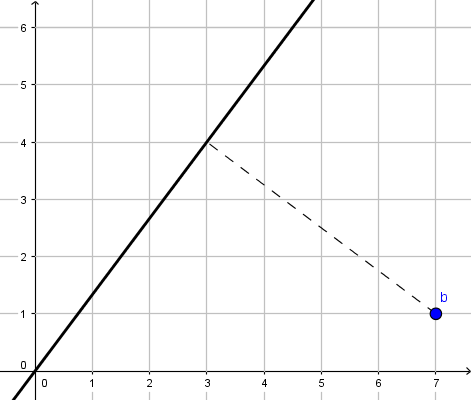
\includegraphics{left_inverse}
\caption{The geometry of equation \ref{impossible_equation}}
\label{fig:left_inverse}
\end{figure}

Using the general notation, here $A=\begin{pmatrix}3 \\ 4\end{pmatrix}\in\mathbb{R}^{2\times 1}$ has rank 1, and so a left inverse can be found:
\begin{equation}
A^{-1}_L=(A^t A)^{-1}A^t=\left(\begin{pmatrix}3 & 4\end{pmatrix}\begin{pmatrix}3 \\ 4\end{pmatrix}\right)^{-1}\begin{pmatrix}3 & 4\end{pmatrix}=\frac{1}{25}\begin{pmatrix}3 & 4\end{pmatrix}
\end{equation}
The best approximation to a solution is then:
\begin{equation}
x=A^{-1}_L b=\frac{1}{25}\begin{pmatrix}3 & 4\end{pmatrix}\begin{pmatrix}7 \\ 1\end{pmatrix}=\frac{21+4}{25}=1
\end{equation}
So, the actual point in the image space is:
\begin{equation}
Ax=\begin{pmatrix}3 \\ 4\end{pmatrix}1=\begin{pmatrix}3 \\ 4\end{pmatrix}
\end{equation}

\subsection{Right inverses}
Similarly, if $A\in\mathbb{R}^{m\times n}$ has rank $m$, then the image space is all of $\mathbb{R}^m$, and hence the corresponding linear transformation is surjective. This means that the equation $Ax=b$ always has a solution, and it will have infinitely many if $n>m$ (as we will see below). The matrix $AA^t$ has rank $m$ as well, and hence is invertible. Analogously, we can use this to construct a right inverse:
\begin{equation}
A^{-1}_R=A^t(AA^t)^{-1},\qquad AA^{-1}_R=AA^t(AA^t)^{-1}=I_m
\end{equation}
This means that $x_s=A^{-1}_R b$ is a solution.

To get an intuition for which $x$ is picked out, consider instead the equation $Ax=0$. The solution space $S$ is the null space of $A$. According to the rank-nullity theorem $S$ has dimension $s=m-n$. Let $l_1,l_2,\cdots,l_s$ be a basis for $S$. These are collected into the $s\times n$ matrix $L$:
\begin{equation}
L=\begin{pmatrix}
| & | & \cdots & | \\
l_1 & l_2 & \cdots & l_s \\
| & | & \cdots & |
\end{pmatrix}
\end{equation}
Now, since we have one solution to the equation $Ax=b$, namely $x_s$, it follows that any vector of the form $s_x+s$, where $s\in S$ is a solution. But this is exactly the affine space $W=x_s+S$ as described in the section on projection above. We now ask: What is the projection of the zero vector onto $W$? According to equation \ref{affine_projection_0} it is:
\begin{equation}
P_W 0=(I-(L^t L)^{-1}L^t)w
\end{equation}
Here $w$ is a vector in $W$. We choose $w=x_sA^{-1}_R b=A^t(AA^t)^{-1}b$:
\begin{equation}
P_W 0=(I-(L^t L)^{-1}L^t)A^t(AA^t)^{-1}b
\end{equation}
But since $L^t A^t=(AL)^t=0$ because of $L$'s construction, the giant cross-term between $A$'s and $L$'s vanishes, and we're left with:
\begin{equation}
P_W 0=A^t(AA^t)^{-1}b=x_s
\end{equation}
In other words, the solution obtained by using $A^{-1}_R$ is the projection of the zero vector onto the solution space. This can be characterized as the solution vector with the smallest possible norm.

\subsubsection{Example}
Consider the equation:
\begin{equation}
\label{many_solutions}
\begin{pmatrix}1 & 1\end{pmatrix}\begin{pmatrix}x \\ y\end{pmatrix}=4
\end{equation}
This clearly has infinitely many solutions, as it is equivalent to $x+y=4$ or $y=-x+4$. Let's consider the right inverse of $A=\begin{pmatrix}1 & 1\end{pmatrix}$:
\begin{equation}
A^{-1}_R=A^t(AA^t)^{-1}=\begin{pmatrix}1 \\ 1\end{pmatrix}\left(\begin{pmatrix}1 & 1\end{pmatrix}\begin{pmatrix}1 \\ 1\end{pmatrix}\right)^{-1}=\frac{1}{2}\begin{pmatrix}1 \\ 1\end{pmatrix}
\end{equation}
Hence, the solution picked out by $A^{-1}_R$ is:
\begin{equation}
\begin{pmatrix}x \\ y\end{pmatrix}=A^{-1}_R b=\frac{1}{2}\begin{pmatrix}1 \\ 1\end{pmatrix}4=\begin{pmatrix}2 \\ 2\end{pmatrix}
\end{equation}
The situation is shown in figure \ref{fig:right_inverse}.

\begin{figure}
\centering
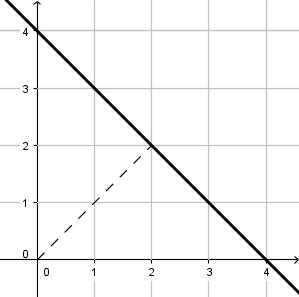
\includegraphics{right_inverse}
\caption{The geometry of equation \ref{many_solutions}}
\label{fig:right_inverse}
\end{figure}

\subsection{Reflexive, generalized inverses}
Both of of these inverses (when they exist) satisfies equation \ref{generalized_inverse}. They also satisfy \ref{reflexive_generalized_inverse}. For instance:
\begin{equation}
A^{-1}_L AA^{-1}_L=(A^t A)^{-1}A^t A(A^t A)^{-1}A^t=(A^t A)^{-1}A^t=A^{-1}_L
\end{equation}
So both are reflexive, generalized inverses.

\section{The Moore-Penrose pseudoinverse}
The \textit{Moore-Penrose pseudoinverse} or simply the pseudoinverse of a real matrix $A$ is the reflexive, generalized inverse $A^+$ which also satisfies:
\begin{equation}
\label{moore-penrose}
(AA^+)^t=AA^+,\qquad(A^+ A)^t=A^+ A
\end{equation}
In other words, for which $AA^+$ and $A^+ A$ are symmetrical\footnote{If $A$ has complex entries, the condition instead becomes that $A$ should be Hermitian.}. Summing it all up, the pseudoinverse has to satisfy the following four conditions:
\begin{enumerate}
\item $AA^+ A=A$
\item $A^+ AA^+=A^+$
\item $(AA^+)^t=AA^+$
\item $(A^+ A)^t=A^+ A$
\end{enumerate}
\subsection{Uniqueness}
If such a pseudoinverse exists, it is unique (hence our use of definite article above). To show this, let $B_1$ and $B_2$ be pseudoinverses of $A$. Then:
\begin{align}
AB_1=(AB_1)^t=B_1^t A^t=B_1^t(AB_2 A)^t=B_1^t A^t B_2^t A^t=&\\
(AB_1)^t(AB_2)^t=AB_1 AB_2=&AB_2
\end{align}
Similarly:
\begin{align}
B_1A=(B_1A)^t=A^t B_1^t=(AB_2 A)^t B_1^t=A^t B_2^t A^t B_1^t=&\\
(B_2 A)^t(B_1 A)^t=B_2 A B_1 A=&B_2 A
\end{align}
But then:
\begin{equation}
B_1=B_1 AB_1=B_2 AB_1=B_2 AB_2=B_2
\end{equation}

\subsection{Intuition behind the pseudoinverse}
The idea behind the pseudoinverse is similar to the one used in singular value decomposition: The dimension of the column and row spaces of a matrix $A\in\mathbb{R}^{m\times n}$ have the same dimension, $r$. So if $y\in\mathbb{R}^m$ is in the column space, there is exactly one vector $x\in\mathbb{R}^n$ so that $Ax=y$. However, for $y$ in the left null space, we're in trouble. But what if we just send these these vectors to the zero vector? This corresponds to projecting onto the column space.

\subsection{Definition for diagonal matrices}
Let $D$ be a diagonal, but not necessarily square matrix, i.e. $D\in\mathbb{R}^{m\times n}$. The diagonal entries are denoted $d_i$. So $D_{ij}=d_i\delta_{ij}$. Following the intuition section, we will set the pseudoinverse of $D$ to be the diagonal $n\times m$ matrix whose diagonal entries are set equal to:
\begin{equation}
d_i^+=
\begin{cases}
0\textrm{ for }d_i=0 \\
\frac{1}{d_i}\textrm{ otherwise}
\end{cases}
\end{equation}
We can use this to write the entries of $D^+$ as $D^+_{ij}=(D_{ji})^+=d_i^+\delta_{ij}$.

\subsubsection{Checking the axioms}
We must now check that the four points above are satisfied:
\begin{enumerate}
\item Calculate the indices of $DD^+ D$:
\begin{equation}
(DD^+ D)_{ij}=\sum_{k=1}^n\sum_{l=1}^m D_{ik}D^+_{kl}D_{lj}=\sum_{k=1}^n\sum_{l=1}^m d_i\delta_{ik}d_k^+\delta_{kl}d_l\delta_{lj}
\end{equation}
Two of the deltas cancel out, so:
\begin{equation}
(DD^+ D)_{ij}=d_i d^+_i d_i\delta_{ij}
\end{equation}
Now, consider the product of the first two terms:
\begin{equation}
\label{pseudo_diagonal}
d_i d^+_i=
\begin{cases}
0\textrm{ if }d_i=0 \\
1\textrm{ if }d_i\neq 0
\end{cases}
\end{equation}
Multiplying by $d_i$ we get $d_i$ in both cases, and so:
\begin{equation}
(DD^+ D)_{ij}=d_i\delta_{ij}
\end{equation}

\item Using the same strategy:
\begin{equation}
(D^+ DD^+)_{ij}=\sum_{k=1}^m\sum_{l=1}^m D^+_{ik}D_{kl}D^+_{lj}=\sum_{k=1}^n\sum_{l=1}^m d_i^+\delta_{ik}d_k\delta_{kl}d_l^+\delta_{lj}
\end{equation}
Again, two deltas cancel:
\begin{equation}
(D^+ DD^+)_{ij}=d_i^+ d_i d_i^+\delta_{ij}
\end{equation}
By using equation \ref{pseudo_diagonal} again we get:
\begin{equation}
(D^+ DD^+)_{ij}=d_i^+\delta_{ij}
\end{equation}

\item Same strategy:
\begin{align}
(DD^+)^t_{ij}=(DD^+)_{ji}&=\sum_{k=1}^n D_{jk}D^+_{ki}=\sum_{k=1}^n d_j\delta_{jk}d^+_k\delta_{ki}=d_i d^+_i\delta_{ij}&=\\
d^+_i d_i\delta{ij}=\sum_{k=1}^m d^+_i\delta_{ik}d_k\delta_{kj}&=\sum_{k=1}^m D_{ik}D^+_{kj}=(DD^+)_{ij}
\end{align}

\item Analogous to 3.
\end{enumerate}

\subsection{Definition for arbitrary matrices}
We can now use the singular value decomposition to generalize the pseudoinverse. If $A\in\mathbb{R}^{m\times n}$ is an arbitrary matrix, then we may write $A=UD V^t$ as above. Now, we set the psuedoinverse to:
\begin{equation}
A^+=VD^+ U^t
\end{equation}

\subsection{Checking the axioms}
We can now show that this definition obeys the four axioms above. Each of the proofs hinge on the result for diagonal matrices:
\begin{enumerate}
\item $AA^+ A=UDV^t VD^+ U^t UDV^t=UDD^+ DV^t=UDV^t=A$
\item $A^+ AA^+=VD^+ U^t UDV^t VD^+ U^t=VD^+ DD^+ U^t=VD^+ U^t=A^+$
\item $(AA^+)^t=(UDV^t VD^+ U^t)^t=(UDD^+ U^t)=$ \\
$U(DD^+)^t U^t= UDD^+ U^t=UDV^t VD^+ U^t=AA^+$
\item $(A^+A)^t=(VD^+ U^t UDV^t)^t=(VD^+ DV^t)=$ \\
$V(D^+ D)^t V^t=VD^+ DV^t=VD^+ U^t UDV^t=A^+ A$
\end{enumerate}

\subsection{Left and right inverses as pseudoinverses}
In the previous section, we looked at left and right inverses as projection operators used for getting the best solution to linear equation systems. It turns out, that these are in fact the pseudoinverse of $A$ in their respective cases. This is done by checking that they satisfy the four axioms. The result then follows by the uniqueness of the pseudoinverse.

\subsubsection{Left inverses}
As above, for $A$ injective, we set $A_L=(A^t A)^{-1}A^t$. We need to show the four axioms are satisfied:
\begin{itemize}
\item $AA_L A=A(A^t A)^{-1}A^t A=A$.
\item $A_L AA_L=(A^t A)^{-1}A^t A(A^t A)^{-1}A^t=(A^t A)^{-1}A^t=A_L$.
\item $(AA_L)^t=(A(A^t A)^{-1}A^t)^t=A(A^t A)^{-1}A^t=AA_L$.
\item $(A_L A)^t=I^t=I=A_L A$.
\end{itemize}

\subsubsection{Right inverses}
Similarly, when $A$ is surjective, we set $A_R=A^t(AA^t)^{-1}$. As above, we need to show it satisfies the four axioms:
\begin{itemize}
\item $AA_R A=AA^t(AA^t)^{-1}A=A$.
\item $A_R AA_R=A^t(AA^t)^{-1}AA^t(AA^t)^{-1}=A^t(AA^t)^{-1}=A_R$.
\item $(AA_R)^t=(AA^t(AA^t)^{-1})^t=I^t=I=AA_R$.
\item $(A_R A)^t=(A^t(AA^t)^{-1}A)^t=A^t(AA^t)^{-1}A=A_R A$.
\end{itemize}

\subsection{Pseudoinverses as limits}
The pseudoinverse can also be found through limit procedures:
\begin{equation}
A^+=\lim_{\delta\rightarrow 0^+}(A^t A+\delta I)^{-1}A^t=\lim_{\delta\rightarrow 0^+}A^t(AA^t+\delta I)^{-1}
\end{equation}
To see why this is true, consider the singular value decomposition for $A$ and $A^t$:
\begin{equation}
A=U\Sigma V^t,\quad A^t=V\Sigma U^t
\end{equation}
This is not strictly true: In general, the sigma matrices will have differing sizes, but since the only true difference is that one has more zeroes in the diagonal than the other, we will slightly abuse notation and use the same symbol for each. Now the above means that:
\begin{equation}
AA^t=U\Sigma V^t V\Sigma U^t=U\Sigma U^t,\quad
A^t A=V\Sigma U^t U\Sigma V^t=V\Sigma^2 V^t
\end{equation}
Now consider the matrix to be inverted in the first limit formula:
\begin{equation}
A^t A+\delta I=V\Sigma^2 V^t+\delta VV^t=V(\Sigma^2+\delta)V^t
\end{equation}
Hence, the eigenvalues of the matrix are:
\begin{equation}
\lambda_i=\frac{1}{\sigma_i^2+\delta}
\end{equation}
Since $\sigma_i^2$ is non-negative, and $\delta$ is positive, this means that all eigenvalues are positive, and hence the inverse exists. Collecting all these eigenvalues into a diagonal matrix $\Lambda$ this means that the inverse can be written $V\Lambda^{-1}V^t$. Now multiply by $A^t$:
\begin{equation}
(A^t A+\delta I)^{-1}A^t=V\Lambda^{-1}V^t V\Sigma U^t=V\Lambda^{-1}\Sigma U^t
\end{equation}
This is a singular value decomposition, with singular values:
\begin{equation}
\frac{\sigma_i}{\sigma_i^2+\delta}
\end{equation}
As $\delta\rightarrow 0^+$ we get $1/\sigma_i$, unless $\sigma_i=0$, then we get zero. This means that we get exactly what the recipe for constructing the pseudoinverse said!

The second limit formula follows from a completely analogous argument.

\section{Principal component analysis}
\textit{Principal component analysis} (or simply PCA) is an algorithm that achieves lossy compression of the information in a data set using SVD.

\subsection{Singular value decomposition of data}
Let $X$ be an $n\times p$ matrix containing $p$ data points of dimensionality $n$. We will assume that the data has been \textit{normalized}, so that the average of each of the $n$ dimensions is zero. In this case, we may write the empirical covariance matrix as:
\begin{equation}
\label{empirical_covariance}
C=\frac{X^t X}{n-1}
\end{equation} 
But, we may also do a singular value decomposition of $X$:
\begin{equation}
\label{data_svd}
X=USV^t
\end{equation}
Inserting equation \ref{data_svd} into \ref{empirical_covariance} we get:
\begin{equation}
C=\frac{1}{n-1}VSU^t USV^t=\frac{1}{n-1}VS^2 V^t
\end{equation}
So, the relationship between the eigenvalues of the covariance matrix and the singular values of $S$ are:
\begin{equation}
\lambda_i=\frac{1}{n-1}s_i^2
\end{equation}
The orthogonal set of rows vectors of $V$ are called \textit{principal axes} and the corresponding \textit{principal components} are the rows of $XV=USV^t V=US$.

\subsection{Autoencoders}
An \textit{autoencoder} of a set of data points $x_1,\cdots, x_p\in\mathbb{R}^n$ consists of two parts:
\begin{itemize}
\item A \textit{coder} function $f: \mathbb{R}^n\rightarrow\mathbb{R}^m$, which turns an input vector $x\in\mathbb{R}^n$ into an encoded vector $c=f(x)\in\mathbb{R}^m$.
\item A \textit{decoder} function $g: \mathbb{R}^m\rightarrow\mathbb{R}^n$ which transforms encoded vectors back into vectors from the original space $\mathbb{R}^n$.
\end{itemize}
The coder and decoder should ideally be chosen such that for an input $x$, we get the exact input back when we decode the coded input. In this case the autoencoder is \textit{lossless}:
\begin{equation}
\forall i:\ g(f(x_i))=x_i
\end{equation}
Here, we will consider \textit{lossy} compression, where this is only approximately true:
\begin{equation}
\forall i:\ g(f(x_i))\approx x_i
\end{equation} 
What this means exactly will vary according to the approach taken.

\subsection{Linear decoder}
Here, we will require the decoder to be linear. Hence it can be expressed in matrix form:
\begin{equation}
g(c)=Dc,
\end{equation}
where $D\in\mathbb{R}^{n\times m}$. This means that the decoded vectors lie in a subspace of $\mathbb{R}^n$ with a dimension of $m$ or less - in the following we assume this dimension to be $m$. We can think of the coded vector $c$ as coordinates for the basis specified by the rows of $D$. There will be several ways to choose the same transformation, so we must expect to restrict the structure of $D$ somehow. More on that below.

Now, consider a coded vector $c=f(x)$. A sensible way to choose $D$ is to require that the squared distance between $x$ and $g(f(x))=Dc$ to be as small as possible. I.e. we seek to minimize:
\begin{align}
||Dc-x||^2=&(Dc-x)^t(Dc-x)=(c^t D^t-x^t)(Dc-x)=\\
&c^t D^t Dc-c^t D^tx-x^t Dc+x^t x
\end{align}
Which encoding minimizes this distance? Let's find out by differentiating with respect to $c$:
\begin{equation}
\frac{\partial ||Dc-x||^2}{\partial c}=2D^t Dc-D^t x-D^t x=2(D^t Dc-D^t x)
\end{equation}
This is zero when:
\begin{equation}
D^t Dc-D^t x=0\Leftrightarrow c=(D^t D)^{-1} D^t x
\end{equation}
So the optimal encoding in this sense will be linear as well. This means that the entire coding/decoding can be written as:
\begin{equation}
g(f(x))=D(D^t D)^{-1} D^t x
\end{equation}
I.e. an orthogonal projection on the image space of $D$.

Now, it is an obvious choice to require the row vectors of $D$ to be orthogonal, as it simplifies the projection operator to $DD^t$:
\begin{equation}
g(f(x))=DD^t x
\end{equation}
This constraint can be written as $D^t D=I_m$.

\subsection{Full data set}
This is just one data point however. We have $p$ such points. Because of the linearity we can conveniently write the encoding of all $p$ points in one matrix equation:
\begin{equation}
g(f(X))=DD^t X\in\mathbb{R}^{n\times p}
\end{equation}
To get the differences between this and the original points, subtract $X$:
\begin{equation}
\Delta=X-DD^t X=(I_n-DD^t)X
\end{equation}
We may view this matrix as $p$ row vectors of differences:
\begin{equation}
\Delta=
\begin{pmatrix}
| & \cdots & | \\
\delta_1 & \cdots & \delta_p \\
| & \cdots & |
\end{pmatrix}
\end{equation}
We wish to minimize to total, squared distance. To get this, consider the following product:
\begin{equation}
\Delta^t \Delta=
\begin{pmatrix}
- & \delta_1^t & -\\
\vdots & \vdots & \vdots \\
- & \delta_p^t & -
\end{pmatrix}
\begin{pmatrix}
| & \cdots & | \\
\delta_1 & \cdots & \delta_p \\
| & \cdots & |
\end{pmatrix}
\end{equation}
So each entry is a dot product between differences, $[\Delta^t \Delta]_{ij}=\delta_i^t\delta_j$. However, we're only interested in the cases where $i=j$. Which means we need to sum over the diagonal: We seek to minimize the \textit{trace} of $\Delta^t \Delta$. However, $\Delta^t \Delta$ can also be written as:
\begin{equation}
X^t(I_n-DD^t)^t(I_n-DD^t)X=X^t(I_n-DD^t)(I_n-DD^t)X=X^t(I_n-DD^t)X
\end{equation}
Here we've used that since $DD^t$ is a projection operator, so is $I_n-DD^t$. Hence it is idempotent. The trace is:
\begin{equation}
\textrm{tr}[X^t(I_n-DD^t)X]=\textrm{tr}[X^tX]-\textrm{tr}[X^t DD^t X]
\end{equation}
The first term is just a constant. This means that the problem reduces to maximizing $\textrm{tr}[X^t DD^t X]$, still subject to $D^t D=I_m$.

\subsection{Solving the optimization problem}
This problem can be solved by induction over $m$. First consider the case where $m=1$. Here $D=d\in\mathbb{R}^{n\times 1}$. The constraint is $d^t d=1$.

A constrained optimization problem such as this can be solved using \textit{Lagrange multipliers}. Here, the constraints can be written as $m^2$ equations:
\begin{equation}
d_i^t d_j=\delta_{ij}\Leftrightarrow d_i^t d_j-\delta_{ij}=0
\end{equation}
Here $d_i$ is the $i$'s row vector of $D$.

\end{document}